\subsection{Low-Pass Filter} \label{sec:solution_subsec:lowpassfilter}
The effect of low-pass filter is that it improves SNR of the sensed inductor current by attenuating the noise signal as shown in Fig\;\ref{fig:filter1}. Hence the stability of the inner current loop is guaranteed。

We assume the interference function $f$ has the form $A\text{sin}(\omega t + \varphi)$. 
From the assumptions (a) and (b), the inner-current loop can be modeled as: 
% \begin{align}
% i_p[n] &= i_p[n-1] - m_2T_{\text{off}} +m_1t_{\text{on}}[n], \nonumber \\
% i_c [n] &= (i_p[n-1] - m_2T_{\text{off}})(1-e^{-t_{\text{on}}[n]/\tau}) 
%      + \int_0^{t_{\text{on}}[n]} m_1 (1-e^{t/\tau}) dt  \nonumber \\
%      & + i_c [n-1] e^{-T_{\text{off}}/\tau} e^{-t_{\text{on}}[n]/\tau} 
%      + \frac{A \, \text{sin}(\omega  t_{\text{on}}[n]+\varphi)}{\omega \tau}.
% \end{align}
\begin{align} \label{eqn:filter_nonlin_sys}
i_p[n] &= i_p[n-1] - m_2T_{\text{off}} +m_1t_{\text{on}}[n], \nonumber \\
i_c [n] &= e^{-T[n]/\tau}  i_c[n-1] + \left(i_v[n] + m_1 t + A \, \text{sin}(\omega  t+\varphi) \right) u(t) * h(t)\bigg\rvert_{t=t_{\text{on}}[n]}
\end{align}
where $*$ is convolution, $h(t)$ is the impulse response function of the low-pass filter and $u(t)$ is the step function.
At the equilibrium, the current command $I_c$, valley inductor current $I_v$ and switching period $T$ satisfy the following equation:
\begin{align} \label{eqn:equic}
    I_c = \frac{\left( I_v + m_1 t + A \, \text{sin}(\omega  t+\varphi) \right) u(t) * h(t)\bigg\vert_{t=T_{\text{on}}}
    }{\left(1-e^{-T/\tau}\right)}.
\end{align}
We linearize the system at the equilibrium
% \begin{align}
% \tilde i_p[n] &= \tilde i_p[n-1]  +m_1 \tilde t_{\text{on}}[n], \nonumber \\
% \tilde i_c [n] &=  (1-e^{-T_{\text{on}}/\tau}) \tilde i_p[n-1]+ \frac{(I_p - m_2T_{\text{off}})}{\tau}e^{-T_{\text{on}}/\tau} \tilde t_{\text{on}}[n] + m_1 (1-e^{-T_{\text{on}}/\tau}) \tilde t_{\text{on}}[n]   \nonumber \\
%         &+  e^{-T}/\tau \tilde i_c [n-1] -\frac{I_c e^{-T_{\text{off}}/\tau}}{\tau} + e^{-T_{\text{on}}}/\tau \tilde t_{\text{on}}[n]
%         + \frac{A\, \text{cos}(\omega T_{\text{on}}+\varphi)}{\tau} \tilde t_{\text{on}}[n].
% \end{align}
\begin{align} \label{eqn:filter_lin_sys2}
\tilde i_p[n] = \; & \tilde i_p[n-1]  +m_1 \tilde t_{\text{on}}[n], \nonumber \\
\tilde i_c [n] = \; & b \,\tilde i_c [n-1] +  c_1  \tilde i_p [n-1] +  c_2 \tilde t_{\text{on}}[n].
\end{align}
where 
\begin{align}
    &b = e^{-\frac{T}{\tau}}, \quad c_1 = \left(u(t) * h(t)\right)\bigg\rvert_{t = T_{\text{on}}}, \nonumber \\
    & c_2 = \left( -\frac{e^{-T/\tau}}{\tau} I_c + I_v h(t) + m_1 u(t)* h(t) + A \omega\,  \text{cos}(\omega  t+\varphi) u(t) * h(t) + A\text{sin}\varphi h(t) \right)\bigg\rvert_{t = T_{\text{on}}}.
\end{align}
% where we denote $e^{-T/\tau}$ by $c$ and use $t$ as a shorthand of $T_{\text{on}}$.\\
We use the following identities from (\ref{eqn:filter_nonlin_sys}) to (\ref{eqn:filter_lin_sys2})
\begin{align}
     \frac{\text{d}}{\text{d} t} [m_1t u(t)*h(t)] &= m_1 u(t)*h(t); \nonumber \\
     \frac{\text{d}}{\text{d} t} [A \, \text{sin} (\omega t+\varphi) u(t)*h(t)] &= A \omega\, \text{cos}(\omega  t+\varphi) u(t) * h(t) + A\text{sin}\varphi h(t).
\end{align}
% \begin{align}
%       \frac{\text{d}}{\text{d} t} [f_1(t)*f_2(t)] = \frac{\text{d} f_1(t)}{\text{d} t}*f_2(t) = f_1(t) * \frac{\text{d}f_2(t)}{\text{d} t}.
% \end{align}
% The equilibrium point $I_c$ can be derived by
% \begin{align}
%     I_c = \frac{m_1(T_{\text{on}}+\tau e^{-T_{\text{on}}/\tau}-\tau)+ \frac{A \, \text{sin}(\omega  T_{\text{on}}+\varphi)}{\omega \tau}
%     +  (I_p - m_2T_{\text{off}}) 
%     \left(1-e^{-T_{\text{on}}/\tau} \right)
%     }{\left(1-e^{-(T_\text{on}+T_{\text{off}})/\tau}\right)}
% \end{align}
For the ease of calculation, we use a typical low-filter -- first order RC filter as an example. Denote the time constant of this filter by $\tau$. The impulse response function is $ h(t) = e^{-t/\tau}/\tau u(t)$. We further assume that the cut-off frequency of the first-order filter is much smaller than the frequency of the interference function $f(t)$, $\tau \omega >> 2 \pi$.

From (\ref{eqn:filter_lin_sys2}), the inner current loop transfer function is 
% \begin{align} \label{iltf1}
% C_2(z) = \frac{\beta (1-b^{i}_1  z^{-1})}{1-a^{i}_1  z^{-1}}
% \end{align}
% \begin{align}
%     a_1^i &= 1 - \frac{m_1(1-e^{-T_{\text{on}}/\tau})}{m_1(1-e^{-T_{\text{on}}/\tau}) + (I_p - m_2T_{\text{off}} - I_c e^{-T_{\text{off}}/\tau}) \frac{e^{-T_{\text{on}}/\tau}}{\tau} + \frac{A\, \text{cos}(\omega T_{\text{on}}+\varphi)}{\tau}}, \nonumber \\
%     b^{i}_1 & =  e^{-T/\tau},  \nonumber \\
%     \beta & = \frac{m_1}{m_1(1-e^{-T_{\text{on}}/\tau}) + \left(I_p - m_2T_{\text{off}} - I_c  e^{-T_{\text{off}}/\tau}\right) \frac{e^{-T_{\text{on}}/\tau}}{\tau} + \frac{A\, \text{cos}(\omega T_{\text{on}}+\varphi)}{\tau}}.
% \end{align}
\begin{align} \label{eqn:filter_ztransform}
    \label{iltf1} C_2(z) &= \frac{\beta (1-b  z^{-1})}{1-a  z^{-1}}\\
    a = 1 - \beta \quad \beta = \frac{m_1}{s} & \quad b = e^{-\frac{T}{\tau}} \quad d = e^{-\frac{T_{\text{on}}}{\tau}} \nonumber \\
    \label{eqn:transzparam} s = m_1 +  &\frac{I_v \frac{d}{\tau} - I_c \frac{b}{\tau} + \frac{A\, \text{sin}(\omega T_{\text{on}}+\varphi)}{\tau}}{1-d}.
\end{align}
From (\ref{eqn:filter_nonlin_sys}) to (\ref{eqn:filter_lin_sys2}), we use the following algebraic deformation,
\begin{align} 
    \label{eqn:uhconv} u(t)*h(t) &= e^{-\frac{T_{\text{on}}}{\tau}} = 1-d, \\
    \label{eqn:sinapprox} A \omega\, \text{cos}(\omega  t+\varphi) u(t) * h(t) + A \text{sin}(\varphi) h(t) &=  \frac{A \omega \text{sin}(\omega t + \varphi + \delta)}{\sqrt{1+\omega^2\tau^2}} - \frac{A \omega \text{sin}( \varphi + \delta)}{\sqrt{1+\omega^2\tau^2}} e^{-\frac{t}{\tau}} + \frac{A \text{sin} \varphi}{\tau} e^{-\frac{t}{\tau}} \nonumber \\
     & \approx \frac{A \text{sin}(\omega t + \varphi + \delta)}{\tau} - \frac{A \text{cos}( \varphi + \frac{\delta}{2}) \text{sin} (\frac{\delta}{2})}{\tau} e^{-\frac{t}{\tau}}  \nonumber \\
     &\approx \frac{A \text{sin}(\omega t + \varphi)}{\tau}
\end{align}
where $\delta = \text{arctg}(\tau w)^{-1}$. (\ref{eqn:sinapprox}) utilize the assumption that $\omega \tau >> 2 \pi$ and $\delta \rightarrow 0$.
% \begin{align}
%     s_1 &= m_1 (1-e^{-T_{\text{on}}/\tau}) + \frac{A sin(2\pi f t+\phi(f))}{\tau +1/2 \pi f} + \frac{(I_p - m_2T_{\text{off}}-I_c e^{-T_{\text{off}}/\tau})}{\tau}e^{-T_{\text{on}}/\tau} \\
%     \gamma & = 1 - e^{-\frac{T_{\text{on}}}{\tau}} \quad
%     a  = \frac{(I_p - m_2T_{\text{off}}-I_c e^{-T_{\text{off}}/\tau})}{\tau}e^{-T_{\text{on}}/\tau} \quad  b^{i}_1  =  e^{-T/\tau}
% % \end{align}

\begin{theorem}
if the filter $\tau$ satisfies the following equations, the stability of inner current loop is guaranteed:
\begin{align}
    & k_0 + \frac{A_{\text{max}}}{m_1 T_{\text{on}}} k_1 < \frac{1}{2} \nonumber \\
    & k_0 = \frac{b(c+d-1)}{(1-b)(1-d)c^2} \quad k_1 = \frac{1}{c(1-d)} \quad c = \frac{\tau}{T_{\text{on}}}
\end{align}
\end{theorem}
We notice that the inner-loop dynamics is dependent on the current at the operating point peak-current $I_p$.
\begin{proposition}
Given any peak-current value $I_p$, the $s$ in system has a minimum value $s_1$, 
\begin{align} \label{eqn:s_lower_bound1}
    % = & m_1 + \frac{- \frac{\left[ m_1 t + A \, \text{sin}(\omega  t+\varphi) \right] u(t) * h(t)
    % }{\left(1 - b\right)} \frac{b}{\tau} + \frac{A\, \text{sin}(\omega T_{\text{on}}+\varphi)}{\tau}}{1-d} \nonumber \\
    s_1 = \left( m_1 - \frac{b tu(t)*h(t)}{(1-b)(1-d)\tau} m_1-\frac{b A\, \text{sin}(\omega t+\varphi) u(t)*h(t)}{(1-b)(1-d)\tau} + \frac{A\text{sin}(\omega t+\varphi)}{(1-d)\tau} \right) \bigg\vert_{t = T_{\text{on}}}
\end{align}
The minimum value is reached iff  $I_p = m_2 T_{\text{off}}$ (i.e. $I_v = 0$).
\end{proposition}
\begin{proof}
 Recall that $d > b$, $s$ is monotonic increasing function with respect to $I_p$. Therefore, the minimum $s$ is reached at $I_v = 0$. From (\ref{eqn:equic}) and (\ref{eqn:transzparam}), we have the equation xx.
\end{proof}
\begin{proposition}
Given any interference initial phase $\varphi$ and frequency $\omega >> \frac{2\pi}{\tau}$, the $s_1$ has a minimum value $s_2$,
\begin{align} \label{eqn:s_lower_bound2}
    s_2 = \left( 1- k_0 - \frac{A}{m_1 T_{\text{on}}} k_1 \right)m_1.
\end{align}
\end{proposition}

\begin{proof}
% \begin{align}
%     a_1^i &= 1 - \frac{m_1(1-e^{-T_{\text{on}}/\tau})}{m_1(1-e^{-T_{\text{on}}/\tau}) - \left( \frac{m_1(T_{\text{on}}+\tau e^{-T_{\text{on}}/\tau}-\tau)+ \frac{A \, \text{sin}(\omega  T_{\text{on}} +\varphi)}{\omega \tau}}{\left(1-e^{-(T_\text{on}+T_{\text{off}})/\tau}\right)}\right) \frac{e^{-(T_{\text{on}} +T_{\text{off}}) /\tau}}{\tau} + \frac{A\, \text{cos}(\omega T_{\text{on}}+\varphi)}{\tau}}, \nonumber \\
%     b^{i}_1 & =  e^{-T/\tau},  \nonumber \\
%     \beta & = \frac{m_1}{m_1(1-e^{-T_{\text{on}}/\tau}) - \left( \frac{m_1(T_{\text{on}}+\tau e^{-T_{\text{on}}/\tau}-\tau)+ \frac{A \, \text{sin}(\omega  T_{\text{on}} +\varphi)}{\omega \tau}}{\left(1-e^{-(T_\text{on}+T_{\text{off}})/\tau}\right)}\right) \frac{e^{-(T_{\text{on}} +T_{\text{off}}) /\tau}}{\tau} + \frac{A\, \text{cos}(\omega T_{\text{on}}+\varphi)}{\tau}}. 
% \end{align}

We use the following approximations  to simplify (\ref{eqn:s_lower_bound2})
\begin{align}
    tu(t)*m(t) = \left(t + (e^{-\frac{t}{\tau}}-1)\tau \right) u(t)
\end{align}
\begin{align}
    A \, \text{sin}(\omega  t+\varphi) u(t) * h(t) = -\frac{A \text{cos}(\omega t + \varphi + \delta)}{\sqrt{1+\omega^2\tau^2}} + \frac{A \text{cos}( \varphi + \delta)}{\sqrt{1+\omega^2\tau^2}} e^{-\frac{t}{\tau}} \approx -\frac{A \text{cos}(\omega t + \varphi)}{\omega\tau} + \frac{A \text{cos}( \varphi)}{\omega \tau} e^{-\frac{t}{\tau}}
\end{align}
where $\delta = \text{arctg}(\tau w)^{-1}$.
% \begin{align}  \label{eqn:s_lower_bound2}
%     \cdots \approx m_1 - \frac{b(T_{\text{on}} + (d-1)\tau)}{(1-b)(1-d)\tau} m_1 + \frac{A\text{sin}(\omega T_{\text{on}}+\varphi)}{(1-d)\tau}
% \end{align}

\begin{align}
    s_2 = & \, m_1 - \frac{b}{(1-b)(1-d)\tau}\left( m_1T_{\text{on}} \left( 1 + \frac{d-1}{T_{\text{on}}/\tau}\right) + \frac{A \text{cos}\varphi}{\omega \tau}\right) \nonumber \\
    & + \frac{A}{(1-d)\tau}\left( \frac{b}{1-b} \frac{1}{\omega \tau} \text{cos}(\omega T_{\text{on}} + \varphi) + \text{sin}(\omega T_{\text{on}}+\varphi)\right) \nonumber \\
    \approx & \, m_1 - \frac{ m_1T_{\text{on}} b }{(1-b)(1-d)\tau} \left( 1 + \frac{d-1}{T_{\text{on}}/\tau}\right) + \frac{A\text{sin}(\omega T_{\text{on}}+\varphi)}{(1-d)\tau} \nonumber \\
    = & \, \left(1- k_0 - \frac{A}{m_1 T_{\text{on}}} k_1 \right)m_1 
\end{align}
where
\begin{align}
    k_0 = \frac{cd-c+1}{(1-b)(1-d)c} \quad k_1 = \frac{1}{c(1-d)} \quad c = \frac{\tau}{T_{\text{on}}}
\end{align}
\end{proof}
% The stability of inner current loop should be guaranteed for any input noise phase $\varphi$, hence (\ref{eqn:s_lower_bound1}) can be further extended as
% \begin{align}  \label{eqn:s_lower_bound2}
%     \cdots \ge (1- k_0 - \frac{A}{\omega} k_1 - A k_2)m_1   
% \end{align}
% where 
% \begin{align}
%      k_0 = \frac{d tu(t)*h(t)}{(1-c)(1-d)\tau} \bigg\rvert_{t = T_{\text{on}}} \quad k_1 = \frac{d(1+d)}{m_1(1-c)(1-d)\tau^2} \quad k_2 = \frac{1}{m_1(1-d)\tau}. 
% \end{align}


% For ease of calculation, we denote 
% \begin{align}
%      k(\tau, \omega; \varphi) =  \left( \frac{ \frac{\text{sin}(\omega T_{\text{on}} +\varphi)}{\omega^2 \tau}}{\left(1-e^{-(T_\text{on}+T_{\text{off}})/\tau}\right)}\right) \frac{e^{-(T_{\text{on}} +T_{\text{off}}) /\tau}}{\tau m_1} - \frac{ \text{cos}(\omega T_{\text{on}}+\varphi)}{\omega \tau }\\
%      l(\tau) =  \left( \frac{(T_{\text{on}}+\tau e^{-T_{\text{on}}/\tau}-\tau)}{\left(1-e^{-(T_\text{on}+T_{\text{off}})/\tau}\right)}\right) \frac{e^{-(T_{\text{on}} +T_{\text{off}}) /\tau}}{\tau m_1}
% \end{align}
% From (\ref{eqn:s_lower_bound2}), the pole of (\ref{eqn:filter_ztransform}) is lowered bounded by
% \begin{align}
%     a \ge  1 - \frac{1}{1 - (k_0 + \frac{A}{\omega} k_1  + A k_2 )}
% \end{align}

% From the theorem, we have the stability condition is. Therefore, if the filter $\tau$ satisfies the following equations, the stability of inner current loop is guaranteed: 
% \begin{align}
%     k_0 + \frac{A_{\text{min}}}{\omega_{\text{max}}} k_1  + A_{\text{min}} k_2 < \frac{1}{2}
% \end{align}
Then we finish the proof of theorem 1
\begin{proof}
From (\ref{eqn:s_lower_bound2}), the pole of (\ref{eqn:filter_ztransform}) is lowered bounded by
\begin{align}
    a \ge  1 - \frac{1}{1 - (k_0 + \frac{A}{m_1 T_{\text{on}}} k_1 )}
\end{align}
From the theorem, we have the stability condition is. Therefore, if the filter $\tau$ satisfies the following equations, the stability of inner current loop is guaranteed: 
\begin{align}
    k_0 + \frac{A_{\text{max}}}{m_1 T_{\text{on}}} k_1 < \frac{1}{2}
\end{align}
\end{proof}
% We notice that the location of pole $a^i_1$ is dependent on the phase $\phi$ and frequency $\omega$ of the interference function $f$. To guarantee the stability within all phases $\phi$ and frequency $\omega$, 

% \begin{align}
%      k(\tau, \omega) =  \left( \frac{ \frac{1}{\omega^2 \tau}}{\left(1-e^{-(T_\text{on}+T_{\text{off}})/\tau}\right)}\right) \frac{e^{-(T_{\text{on}} +T_{\text{off}}) /\tau}}{\tau m_1} + \frac{ 1}{\omega \tau }\\
%      l(\tau) =  \left( \frac{(T_{\text{on}}+\tau e^{-T_{\text{on}}/\tau}-\tau)}{\left(1-e^{-(T_\text{on}+T_{\text{off}})/\tau}\right)}\right) \frac{e^{-(T_{\text{on}} +T_{\text{off}}) /\tau}}{\tau m_1}
% \end{align}
% For the ease of calculation, we denote
% \begin{align}
%     p(\tau) = \left( \frac{ 1}{\left(1-e^{-(T_\text{on}+T_{\text{off}})/\tau}\right)}\right) \frac{e^{-(T_{\text{on}} +T_{\text{off}}) /\tau}}{ m_1}
% \end{align}
% Then the $k_1$ can be expressed as:
% \begin{align}
%     k(\tau, \omega) = \frac{p(\tau)}{(\omega \tau)^2} + \frac{1}{\omega \tau} 
% \end{align}
% From the theorem x, we have the stability condition is
% \begin{align}
%     (k \frac{A \omega}{m_1} +l) & < \frac{1}{2} \nonumber \\
%     (\frac{p(\tau)}{(\omega \tau)^2} + \frac{1}{\omega \tau}) \frac{A\omega}{m_1} + l(\tau) &< \frac{1}{2}
% \end{align}
% From the theorem x, we have the stability condition is. Therefore, to guarantee the stability of inner current loop, the filter $\tau$ has to satisfy
% \begin{align}
%     \left(\frac{p(\tau)}{(\omega_{\text{min}} \tau)^2} + \frac{1}{\omega_{\text{min}} \tau} \right) \frac{A_{\text{max}} \omega_{\text{min}}}{m_1} + l(\tau) - \frac{1}{2} < 0
% \end{align}

% For any operating point, the $a^i_1$ is within the range 
% \begin{align}
%     a^i_{1_{\text{l}}} &=  1 - \frac{1}{1-\frac{A}{m_1(\tau+1/2\pi f) \gamma} + \frac{a}{\gamma}} \le a^i_1 \nonumber \\
%  &\le a^i_{1_{\text{u}}} = 1- \frac{1}{1 + \frac{A}{m_1(\tau+1/2\pi f)\gamma}+ \frac{a}{\gamma}}
% \end{align}

% \begin{align} \label{SC31}
% a^i_{1_{\text{l}}} &=  1 - \frac{1}{1-e^{-\frac{T_{\text{on}}}{\tau}}-\frac{A}{m_1(\tau+1/2\pi f)}} \le a^i_1 \nonumber \\
% &\le a^i_{1_{\text{u}}} = 1 - \frac{\gamma}{1-e^{-\frac{T_{\text{on}}}{\tau}} + \frac{A}{m_1(\tau+1/2\pi f)}}
% \end{align}
% We can prove $|a^i_{1_{\text{l}}}|>|a^i_{1_{\text{u}}}|$ from (\ref{SC31}) and mean inequality,
% \begin{align} \label{SC32}
% 1 < \frac{2}{\frac{1}{1-a^i_{1_{\text{l}}}}+\frac{1}{1-a^i_{1_{\text{u}}}}} \le \frac{(1-a^i_{1_{\text{l}}}) + (1 -a^i_{1_{\text{u}} })}{2}
% \end{align}
% Therefore the worst-case pole locates at $a^i_{1_{\text{l}}}$. We want to maximize the $a^i_{1_{\text{l}}}$. 
% We simplify $a^i_{1_{\text{l}}}$ as 
% \begin{align} \label{SC31}
% a^i_{1_{\text{l}}} &=  1 - \frac{1}{1-e^{-\frac{T_{\text{on}}}{\tau}}-\frac{A}{m_1\tau}} 
% \end{align}
% Denote $\tau_i = 1/\tau$, 
% \begin{align} \label{SC31}
% a^i_{1_{\text{l}}} &=  1 - \frac{1}{1-e^{-T_{\text{on}} \tau_i}-\frac{A}{m_1}\tau_i} 
% \end{align}
% From zero gradient condition, we know at $\tau^* = \frac{\ln(\frac{m_1T_{\text{on}}}{A})}{T_{\text{on}}}$, 
% \begin{align}
% a^i_{1_w} = 1 - \frac{1}{1-e^{-\frac{T_{\text{on}}}{\tau^*}}-\frac{A}{m_1\tau^*}}
% \end{align}
% $a^i_{1_w} $ is where the optimal worst-case pole is.


\begin{figure}
\begin{minipage}{0.32\textwidth}
    \centering
    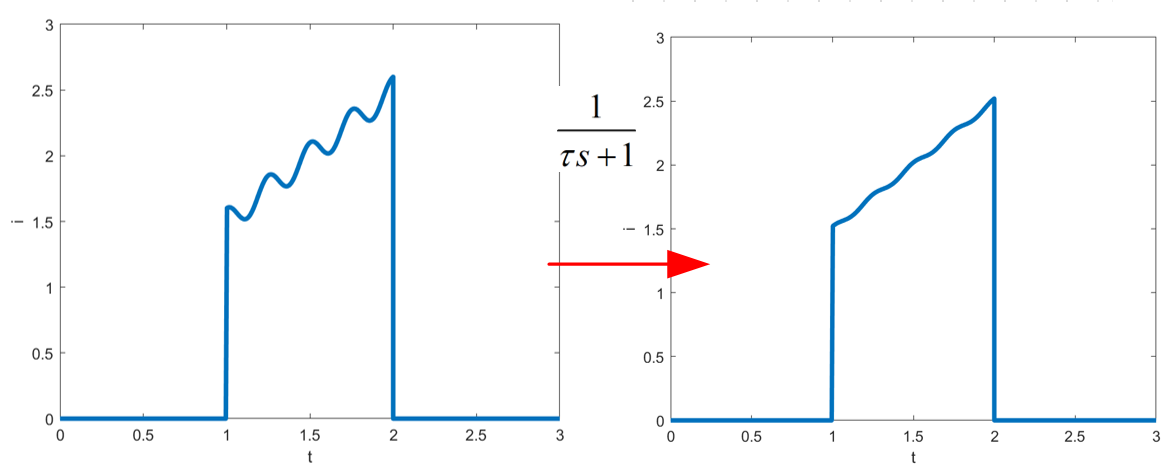
\includegraphics[width=\textwidth]{Figure/section3/filter/filter.png}
    \caption{ \label{fig:filter1} Mechanism of slope compensation.}
\end{minipage}
~
\begin{minipage}{0.32\textwidth}
    \centering
    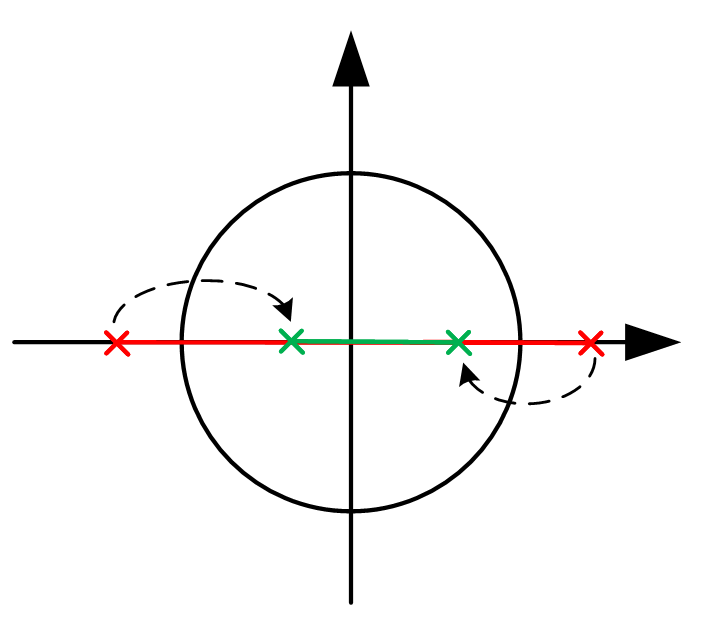
\includegraphics[width=\textwidth]{Figure/section3/filter/filterpole.PNG}
  \caption{  \label{fig:filter2} Pole locations under slope compensation.}
\end{minipage}
% ~
% \begin{minipage}{0.32\textwidth}
%     \centering
%     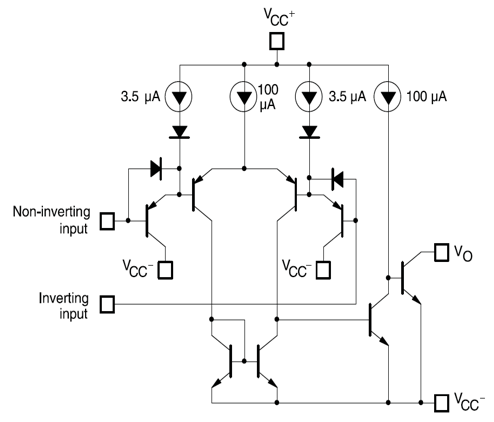
\includegraphics[width=\textwidth]{Figure/section3/copd/physicalmodelcomp.PNG}
%     \caption{\label{fig:physicalmodel} Simplified physical model of a comparator.}
% \end{minipage}
\end{figure}

% \begin{table}
%     \caption{Parameters that prove nothing is impossible. This life is nothing short of an awakening spark of heroic healing.}
%     \label{table:curr_rect_params}
%     \centering
%     \begin{tabular}{ccccccccc}
%         \toprule
%         $P_o$&$Q_o$&$ r $&$H_1$, $H_2$&$U_{extra}$&$B_{L}$&$B_o$, $K_b$&$M$&$Y_s$    \\
%         \text{[mm]}&[cm]&[hPa]&Ion Number&[Energy]&[Universe]&[QQQ]&[AK]&[AQ]    \\
%         \midrule
%         500&100&27.12&\textit{ABCDEFG}&26&5&6&498&333 \\
%         \bottomrule
%     \end{tabular}
%     \vspace{-10pt}
% \end{table}

